% ------------------------------------------------------------------------------
% TYPO3 Version 10.2 - What's New (Dutch Version)
%
% @license	Creative Commons BY-NC-SA 3.0
% @link		https://typo3.org/help/documentation/whats-new/
% @language	Dutch
% ------------------------------------------------------------------------------

\section{Inleiding}
\begin{frame}[fragile]
	\frametitle{Inleiding}

	\begin{center}\huge{Inleiding}\end{center}
	\begin{center}\huge{\color{typo3darkgrey}\textbf{De feiten}}\end{center}

\end{frame}

% ------------------------------------------------------------------------------
% TYPO3 Version 10.2 - The Facts

\begin{frame}[fragile]
	\frametitle{Inleiding}
	\framesubtitle{TYPO3 Versie 10.2 - De feiten}

	\begin{itemize}
		\item Publicatiedatum: 3 december 2019
		\item Publicatietype: Sprint Release
	\end{itemize}

	\begin{figure}
		
\includegraphics[width=0.95\linewidth]{Introduction/typo3-v10-2-banner.png}
	\end{figure}

\end{frame}

% ------------------------------------------------------------------------------
% TYPO3 Version 10.2 - Executive Summary

\begin{frame}[fragile]
	\frametitle{Inleiding}
	\framesubtitle{Managementsamenvatting}

	\small
		TYPO3 versie 10.2 is de derde sprint release op weg naar de LTS-versie
		(long-term support) in 2020. Het is ook de laatste sprint release van dit
		jaar.

		\vspace{0.2cm}

		Tijdens de TYPO3 Initiative Week (T3INIT19) zijn er veel functies ontwikkeld
		en TYPO3 v10.2 bevat reeds een aantal van deze componenten.

		\vspace{0.2cm}

		Deze release maakt de weg vrij voor een hoogstaande omgeving. TYPO3 v10.2 ondersteunt
		niet alleen Symfony versie 5.0, maar het is ook de eerste TYPO3 release die
		PHP versie 7.4 ondersteunt. Daarbij is het de laatste release voor de feature freeze
		release in february 2020.

	\normalsize

\end{frame}

% ------------------------------------------------------------------------------
% System Requirements

\begin{frame}[fragile]
	\frametitle{Inleiding}
	\framesubtitle{Systeemeisen}

	\begin{itemize}
		\item PHP versie 7.2, 7.3 of 7.4
		\item PHP instellingen:

			\begin{itemize}
				\item \texttt{memory\_limit} >= 256M
				\item \texttt{max\_execution\_time} >= 240s
				\item \texttt{max\_input\_vars} >= 1500
				\item compilatieoptie \texttt{-}\texttt{-disable-ipv6} moet \underline{niet} worden gebruikt
			\end{itemize}

		\item De meeste databaseservers die worden ondersteund door \textbf{Doctrine DBAL} werken ook met TYPO3.
			De geteste database systemen zijn:
	\end{itemize}

	\begin{figure}
		
\includegraphics[width=0.80\linewidth]{Introduction/logo-databases.png}
	\end{figure}

\end{frame}

% ------------------------------------------------------------------------------
% Development, Release and Maintenance Timeline

\begin{frame}[fragile]
	\frametitle{Inleiding}
	\framesubtitle{Ontwikkeling-, versie- en onderhouds-tijdlijn}

	\textbf{TYPO3 v10}

	\begin{figure}
		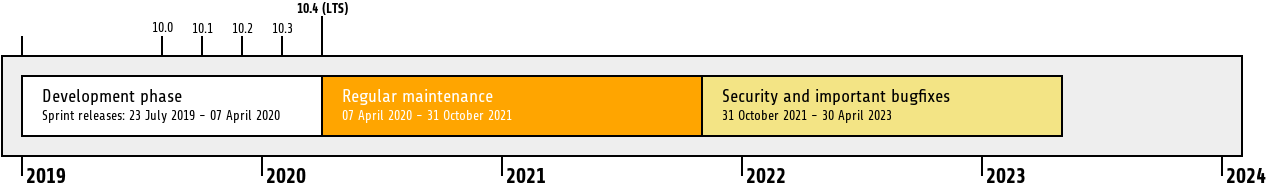
\includegraphics[width=1\linewidth]{Introduction/typo3-v10-lifecycle.png}
	\end{figure}

	\textbf{Verlengde ondersteuning}\newline
	\smaller
		De \href{https://typo3.com}{TYPO3 GmbH} biedt nog extra ondersteuningsopties aan
	    voor TYPO3 v10 LTS, zelfs na 30 april 2023 tot twee jaar lang.
	\normalsize

\end{frame}

% ------------------------------------------------------------------------------
% TYPO3 v10 Roadmap

\begin{frame}[fragile]
	\frametitle{Inleiding}
	\framesubtitle{TYPO3 v10 Roadmap}

	Verwachte verschijningsdata en de focus van de versie:

	\begin{itemize}

		\item v10.0 \tabto{1.1cm}23/juli/2019\tabto{3.4cm}De weg vrijmaken voor spannende nieuwe concepten en API's
		\item v10.1 \tabto{1.1cm}01/okt/2019\tabto{3.4cm}Verbeterde routing en Site behandeling v2
		\item
			\begingroup
				\color{typo3orange}
				v10.2 \tabto{1.1cm}03/dec/2019\tabto{3.4cm}Fluid/Rendering Engine verbeteringen
			\endgroup
		\item v10.3 \tabto{1.1cm}04/feb/2020\tabto{3.4cm}Feature Freeze
		\item v10.4 \tabto{1.1cm}07/apr/2020\tabto{3.4cm}LTS Versie (Long-term Support)

	\end{itemize}

	\smaller
		\url{https://typo3.org/article/typo3-v10-roadmap/}\newline
		\url{https://typo3.org/article/typo3-v10-safe-and-sound/}
	\normalsize

\end{frame}

% ------------------------------------------------------------------------------
% Installation

\begin{frame}[fragile]
	\frametitle{Inleiding}
	\framesubtitle{Installatie}

	\begin{itemize}
		\item Offici\"ele \textit{klassieke} installatieprocedure op Linux/Mac OS X\newline
		(DocumentRoot bijvoorbeeld \texttt{/var/www/site/htdocs}):
\begin{lstlisting}
$ cd /var/www/site
$ wget --content-disposition get.typo3.org/10.2
$ tar xzf typo3_src-10.2.0.tar.gz
$ cd htdocs
$ ln -s ../typo3_src-10.2.0 typo3_src
$ ln -s typo3_src/index.php
$ ln -s typo3_src/typo3
$ touch FIRST_INSTALL
\end{lstlisting}

		\item Symbolische koppelingen op Microsoft Windows:

			\begin{itemize}
				\item Gebruik \texttt{junction} op Windows XP/2000
				\item Gebruik \texttt{mklink} op Windows Vista en Windows 7 of hoger
			\end{itemize}

	\end{itemize}
\end{frame}

% ------------------------------------------------------------------------------
% Installation using composer

\begin{frame}[fragile]
	\frametitle{Installatie en Upgrade}
	\framesubtitle{Installatie met \texttt{composer}}

	\begin{itemize}
		\item Installatie met \textit{composer} onder Linux, Mac OS X en Windows 10:

\begin{lstlisting}
$ cd /var/www/site/
$ composer create-project typo3/cms-base-distribution typo3v10 ^10.1
\end{lstlisting}

		\item Of anders kan een maatwerk \texttt{composer.json} bestand gemaakt worden en dan:

\begin{lstlisting}
$ composer install
\end{lstlisting}

			Een voorbeeld \texttt{composer.json} is te downloaden van:\newline
			\smaller
				\href{https://composer.typo3.org}{https://composer.typo3.org}
			\normalsize

	\end{itemize}
\end{frame}

% ------------------------------------------------------------------------------
